\chapter{Concepts of Wireguard}
  This chapter provide the core concepts of Wireguard protocol, especially in its handshake
  and timer state machine. Section \ref{w1} gives a high-level overview of the traits of the
  protocols, and the cryptography primitives that they build upon. 
  Section \ref{w2}  details the fondational handshake protocol that Wireguard's
  key exchange protocol builds upon. Section \ref{w3} defined all messages types of Wireguard and
  section \ref{w4} descibes the timer state machine.
\section{Protocol \& Cryptography} \label{w1}
\subsection{Overview}
 Wireguard works as an encrypted IP network tunnel, resides at the layer 3 of the OSI layer, and
 uses UDP as its transport protocol. The establishment of a secure session before any 
 transmission of data is via 1-RTT key-exchange handshake protocols. This handshake protocol
 is designed based on a Trevor Perin's noise handshake pattern \cite{noise}. After the handshake, the  
 transported IP payload are protected using ChaCha20-Poly1305 Authenticated Encryption with 
 Associated Data (AEAD) \cite{rfc8439}.

 In Wireguard, the endpoints of communication have no role of server and client, but works in a
 peer-to-peer style. At any point in time, a peer can have a role of an \textbf{initator}, start to send 
 a handshake initiation message to create a secure channel with a \textbf{responder}. If the secure channel
 is not active for some amount of time, the initiator peer can change to a responder in the event of
 a the previous responder tries to initiate a new handshake, leading to the establishment of a new session
 between 2 peers. Figure \ref{fig:pwu_hs} illustrates this handshake flow with periodic key rotation.

\begin{figure}[h]
  \centering
  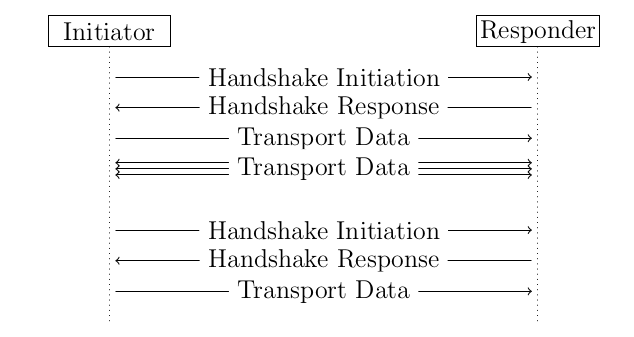
\includegraphics[width=0.8\linewidth]{pwu}
  \caption{After the handshake, both peers can send data towards each other. After a duration, rekeying occurs to create a new session. See \cite[p.~7]{pwu}}
  \label{fig:pwu_hs}
\end{figure}

 A static 32-byte Curve25519 \cite{curve} public key are used to identified an endpoint inside the tunnel. Without the
 proof of sender's knowledge on this public key, an endpoint will never respond. Thus, adversaries can't
 probe any system protected by Wireguard, using port scanning if they do not know the long-term static 
 public key.

The Wireguard handshake protocol can be considered as a 1.5 round-trip time (1.5-RTT) handshake \cite{pwu}. 
Upon the reception of the handshake response after sending a handshake initiation, the initiator
can promplty begin delivering encrypted payload. To safeguard against replay attacks, 
the responder must wait to send encrypted data messages until it has received an encrypted data 
message from the initiator, which serves as an acknowledgment of the handshake response.

During a handshake, new ephemeral key pairs will be generated by both parties, with the private key
being wiped after the handshake, assuring the forward secrecy of the session. Each session is bound
by fixed lifetime and the number of data messages that can be sent. When either of the limits is reached,
the derivation of new session keys are required if the peers want to extend the communication. The impact
of compromised session key is also mitigated by frequent periodic key rotation.

There is no direct shutdown signal within the protocol, only session removal after a fixed duration.
Even if one side has terminated its VPN tunnel, the peer would remain unaware and 
keep forwarding data.

Wireguard also provides an optional pre-shared symmetric key (PSK) mode, where any pairs of peer
pre-share a 256-bit symmetric encryption key between themselves, to assure the post-quantum 
security as long as the PSK never leaks out. This protection is against the idea that if 
adversaries may be recording all the traffic for a long time, until the quantum computer exists.
With PSK, despite the fact they maybe break all Curve25519-encrypted traffic, but not the ones that
include a PSK.

Another adversary model that Wireguard mititage is the denial of service through CPU exhaustion denial
of services attack \cite[p.~268]{cpu}. This mechanism is achieved via an encrypted cookie, when a peer is currently 
under load. This will be explained more in section \ref{iot:cookie}.

At last, Wireguard is cryptographically opinionated. The protocol intentionally does not provide 
any form of flexibility when it comes to choosing the cryptography suite, hence a negation for
cryptography algorithms does not exist. Specifically, Wireguard uses the following modern
cryptography constructions:
\begin{description}
  \item[Noise protocol framework]  A set of cryptographic handshake patterns that 
  serve as building blocks for creating new secure protocols with authenticated key agreement.
  \item[Elliptic Curve Diffie-Hellman (ECDH)] A Curve25519-based key-argeement protocol 
  with small key size and simple requirements regarding key validation.
  \item[ChaCha20-Poly1305] a modern AEAD combining ChaCha20 \cite{chacha20} stream cipher 
  and Poly1305 \cite{poly1305} authenticator to achieve authenticity and confidentiality. 
  \item[XChaCha-Poly1305] an extended version of chacha20-poly1305 that supports 192-bit nonce.
  This is used for cookie encryption \cite{irtf-cfrg-xchacha-03}.
  \item[HKDF] The HMAC-based Key Derivation Function \cite{rfc5869} to derive the encryption
  and decryption keys from the handshake state, keys and protocol messages.
  \item[BLAKE2] A fast and cryptographic hash function for message authentication code and is used
  by the HKDF \cite{rfc7693}.

\end{description}

\subsection{Cryptokey Routing}
  The binding between peers and the allowed source IP addresses is the fundamental principle to build 
  a secure VPN. As mentioned above, in Wireguard, peer must be identified by the 32-byte
  Curve25519 public key, allowing an association between the public key and the set
  of allowed IP addreses on the peer. This simple mapping is the concept behind the cryptokey
  routing table of Wireguard. A transmission of outbound packet will consult this table to search
  for the approriate public key, using the IP destination address of the packet. With inbound packets,
  after decryption and authentication, the source IP address need to be resolved to the same 
  peer that have the same public key used in the secure session for decrypting the packet. 
  In cryptokey routing table, each peer may optionally pre-specify an outer external IP address
  and UDP port of that peer's endpoint. If the endpoint is not specified, the external
  source IP of the machine will be used to determine the endpoint .
  This design also allow the peers to roam freely between different external IP addresses as the
  public is the main identification of the peer.
  
  Combining the roaming and the cryptokey routing table, when the network interface needs
  to send the data out, the flow start with the inspection of the IP destination of the packet 
  to find the corresponding peer and its public key (An ICMP "no route to host" will be returned
  in case of no peer). The packet is then encrypted with mentioned AEAD, prepended with
  extra headers and sent as a UDP packet to the internet. On the receiving flow, when a UDP packet
  is received, Wireguard finds the matching peer, decrypts the packet and updates the peers' endpoint.
  If the packet is either not an IP packet or there is no entry for source IP address of the packet
  inside the cryptokey routing table, the packet is droped. Otherwise, the packet will be dispatched
  to the layer above.
\section{Noise} \label{w2}
\section{Wireguard Messages} \label{w3}
\section{Timers} \label{w4}